% Template for PLoS
% Version 3.5 March 2018
%
% % % % % % % % % % % % % % % % % % % % % %
%
% -- IMPORTANT NOTE
%
% This template contains comments intended 
% to minimize problems and delays during our production 
% process. Please follow the template instructions
% whenever possible.
%
% % % % % % % % % % % % % % % % % % % % % % % 
%
% Once your paper is accepted for publication, 
% PLEASE REMOVE ALL TRACKED CHANGES in this file 
% and leave only the final text of your manuscript. 
% PLOS recommends the use of latexdiff to track changes during review, as this will help to maintain a clean tex file.
% Visit https://www.ctan.org/pkg/latexdiff?lang=en for info or contact us at latex@plos.org.
%
%
% There are no restrictions on package use within the LaTe\times files except that 
% no packages listed in the template may be deleted.
%
% Please do not include colors or graphics in the text.
%
% The manuscript LaTe\times source should be contained within a single file (do not use \input, \externaldocument, or similar commands).
%
% % % % % % % % % % % % % % % % % % % % % % %
%
% -- FIGURES AND TABLES
%
% Please include tables/figure captions directly after the paragraph where they are first cited in the text.
%
% DO NOT INCLUDE GRAPHICS IN YOUR MANUSCRIPT
% - Figures should be uploaded separately from your manuscript file. 
% - Figures generated using LaTe\times should be extracted and removed from the PDF before submission. 
% - Figures containing multiple panels/subfigures must be combined into one image file before submission.
% For figure citations, please use "Fig" instead of "Figure".
% See http://journals.plos.org/plosone/s/figures for PLOS figure guidelines.
%
% Tables should be cell-based and may not contain:
% - spacing/line breaks within cells to alter layout or alignment
% - do not nest tabular environments (no tabular environments within tabular environments)
% - no graphics or colored text (cell background color/shading OK)
% See http://journals.plos.org/plosone/s/tables for table guidelines.
%
% For tables that exceed the width of the text column, use the adjustwidth environment as illustrated in the example table in text below.
%
% % % % % % % % % % % % % % % % % % % % % % % %
%
% -- EQUATIONS, MATH SYMBOLS, SUBSCRIPTS, AND SUPERSCRIPTS
%
% IMPORTANT
% Below are a few tips to help format your equations and other special characters according to our specifications. For more tips to help reduce the possibility of formatting errors during conversion, please see our LaTe\times guidelines at http://journals.plos.org/plosone/s/latex
%
% For inline equations, please be sure to include all portions of an equation in the math environment.  For example, x$^2$ is incorrect; this should be formatted as $x^2$ (or $\mathrm{x}^2$ if the romanized font is desired).
%
% Do not include text that is not math in the math environment. For example, CO2 should be written as CO\textsubscript{2} instead of CO$_2$.
%
% Please add line breaks to long display equations when possible in order to fit size of the column. 
%
% For inline equations, please do not include punctuation (commas, etc) within the math environment unless this is part of the equation.
%
% When adding superscript or subscripts outside of brackets/braces, please group using {}.  For example, change "[U(D,E,\gamma)]^2" to "{[U(D,E,\gamma)]}^2". 
%
% Do not use \cal for caligraphic font.  Instead, use \mathcal{}
%
% % % % % % % % % % % % % % % % % % % % % % % % 
%
% Please contact latex@plos.org with any questions.
%
% % % % % % % % % % % % % % % % % % % % % % % %

\documentclass[10pt,letterpaper]{article}
\usepackage[top=0.85in,left=2.75in,footskip=0.75in]{geometry}

% amsmath and amssymb packages, useful for mathematical formulas and symbols
\usepackage{amsmath,amssymb}

% Use adjustwidth environment to exceed column width (see example table in text)
\usepackage{changepage}

% Use Unicode characters when possible
\usepackage[utf8x]{inputenc}

% textcomp package and marvosym package for additional characters
\usepackage{textcomp,marvosym}

% cite package, to clean up citations in the main text. Do not remove.
\usepackage{cite}

% Use nameref to cite supporting information files (see Supporting Information section for more info)
\usepackage{nameref,hyperref}

% line numbers
\usepackage[right]{lineno}

% ligatures disabled
\usepackage{microtype}
\DisableLigatures[f]{encoding = *, family = * }

% color can be used to apply background shading to table cells only
\usepackage[table]{xcolor}

% array package and thick rules for tables
\usepackage{array}

% create "+" rule type for thick vertical lines
\newcolumntype{+}{!{\vrule width 2pt}}

% create \thickcline for thick horizontal lines of variable length
\newlength\savedwidth
\newcommand\thickcline[1]{%
  \noalign{\global\savedwidth\arrayrulewidth\global\arrayrulewidth 2pt}%
  \cline{#1}%
  \noalign{\vskip\arrayrulewidth}%
  \noalign{\global\arrayrulewidth\savedwidth}%
}

% \thickhline command for thick horizontal lines that span the table
\newcommand\thickhline{\noalign{\global\savedwidth\arrayrulewidth\global\arrayrulewidth 2pt}%
\hline
\noalign{\global\arrayrulewidth\savedwidth}}


% Remove comment for double spacing
%\usepackage{setspace} 
%\doublespacing

% Text layout
\raggedright
\setlength{\parindent}{0.5cm}
\textwidth 5.25in 
\textheight 8.75in

% Bold the 'Figure #' in the caption and separate it from the title/caption with a period
% Captions will be left justified
\usepackage[aboveskip=1pt,labelfont=bf,labelsep=period,justification=raggedright,singlelinecheck=off]{caption}
\renewcommand{\figurename}{Fig}

% Use the PLoS provided BiBTe\times style
\bibliographystyle{plos2015}

% Remove brackets from numbering in List of References
\makeatletter
\renewcommand{\@biblabel}[1]{\quad#1.}
\makeatother



% Header and Footer with logo
\usepackage{lastpage,fancyhdr,graphicx}
\usepackage{epstopdf}
%\pagestyle{myheadings}
\pagestyle{fancy}
\fancyhf{}
%\setlength{\headheight}{27.023pt}
%\lhead{
\includegraphics[width=2.0in]{PLOS-submission.eps}}
\rfoot{\thepage/\pageref{LastPage}}
\renewcommand{\headrulewidth}{0pt}
\renewcommand{\footrule}{\hrule height 2pt \vspace{2mm}}
\fancyheadoffset[L]{2.25in}
\fancyfootoffset[L]{2.25in}
\lfoot{\today}

%% Include all macros below

\newcommand{\sticky}{proglobular~}
\newcommand{\dSNPs}{dSNPs~}
\newcommand{\nSNPs}{nSNPs~}
\newcommand{\dSNP}{dSNP~}
\newcommand{\nSNP}{nSNP~}
\newcommand{\hydrochar}{hydrophobicity class}
\newcommand{\chargechar}{charge class}
\newcommand{\grace}[1]{\textcolor{red}{#1}}
\newcommand{\ruchi}[1]{\textcolor{blue}{#1}}
\newcommand{\matt}[1]{\textcolor{purple}{Matt says: #1}}
\usepackage{makecell}
\usepackage{multirow}

\renewcommand\theadalign{bc}
\renewcommand\theadfont{\bfseries}
\renewcommand\theadgape{\Gape[4pt]}
\renewcommand\cellgape{\Gape[4pt]}

%% END MACROS SECTION



\begin{document}
\vspace*{0.2in}

% Title must be 250 characters or less.
\begin{flushleft}
{\Large
\textbf\newline{Disease associated mutations in intrinsically disordered proteins show evidence of enrichment in hydrophobic blobs} % Please use "sentence case" for title and headings (capitalize only the first word in a title (or heading), the first word in a subtitle (or subheading), and any proper nouns).
}
\newline
% Insert author names, affiliations and corresponding author email (do not include titles, positions, or degrees).
\\
Ruchi Lohia\textsuperscript{1},
Kaitlin Bassi\textsuperscript{1},
Matt Hansen\textsuperscript{2},
Grace Brannigan\textsuperscript{1,3*},
\\
\bigskip
\textbf{1} Center for Computational and Integrative Biology, Rutgers University, Camden, NJ, USA
\\
\textbf{2}  Department of Genetics and Center of Excellence in Environmental Toxicology, University of Pennsylvania 
\\
\textbf{3} Department of Physics, Rutgers University, Camden, NJ, USA
\\
\bigskip

% Insert additional author notes using the symbols described below. Insert symbol callouts after author names as necessary.
% 
% Remove or comment out the author notes below if they aren't used.
%
% Primary Equal Contribution Note
%\Yinyang These authors contributed equally to this work.

% Additional Equal Contribution Note
% Also use this double-dagger symbol for special authorship notes, such as senior authorship.
%\ddag These authors also contributed equally to this work.

% Current address notes
%\textcurrency Current Address: Dept/Program/Center, Institution Name, City, State, Country % change symbol to "\textcurrency a" if more than one current address note
% \textcurrency b Insert second current address 
% \textcurrency c Insert third current address

% Deceased author note
%\dag Deceased

% Group/Consortium Author Note
%\textpilcrow Membership list can be found in the Acknowledgments section.

% Use the asterisk to denote corresponding authorship and provide email address in note below.
* grace.brannigan@rutgers.edu(GB)

\end{flushleft}

\section*{Abstract}
%\cite{ConchilloSole20074}
%The \textbf{consequence of an amino acid substitution} in disordered proteins is difficult to predict. Previously, we developed a novel hierarchical sequence-based framework for analysis and conceptualization of long intrinsically disordered proteins (IDPs). We developed a hierarchical sequence-based framework for analysis and conceptualization, which first identifies “blobs” of 4-15 residues representing local globular regions or linkers. This sequence-based blob decomposition framework was able to predict enrichment of higher-order (tertiary) structure in a disordered protein due to a disease-causing SNP. Here, we extend the sequence classification analysis to 12,508 proteins and 70,297 SNPs, testing for enrichment of disease-associated SNPs within a given protein sequence. We find that disease-associated SNPs are enriched in hydrophobic blobs within the given protein sequence (1.15 fold). Interestingly, for the proteins directly involved in aggregation disease the enrichment is even higher (1.35 fold). We further demonstrate that 20\% of disease mutations cause blob properties transitions, which represents a 1.7 fold increase compared to annotated polymorphisms. Finally, we developed a web tool for interactive identification of sequence topology for any given protein sequence. This work represents the first systematic, bottom-up, attempt to both identify and annotate subdomains within proteins that are enriched for functional effects.

% Please keep the Author Summary between 150 and 200 words
% Use first person. PLOS ONE authors please skip this step. 
% Author Summary not valid for PLOS ONE submissions.   
\section*{Author summary} 
\section*{Introduction}
An ambitious task for human genetics is discovering the genetic basis for heritable traits and disease risks. Genome-wide association studies (GWAS) can identify variants associated with a effect regardless of the genomic or protein context of the variant. Associated variants are often not directly causal but instead passively ``tag'' haplotypes containing the true causal variants that are either unknown or observed but not directly tested for association. The pattern of linkage disequilibrium that defines ``tagging'' is population dependent. Any information on the protein-level function of the local sequence surrounding an associated variant can help fine-map and rank putative causal variants from a list of associations.  

Many bioinformatics approaches apply known principles of protein physical chemistry to the local sequence near the variant, considering effects of the mutation on properties like the residue mass, size, charge, hydrophobicity, C-beta density, and residue flexibility~\cite{Hecht2015, needed}.  Such methods may also rely on known protein structures in order to incorporate properties such as local secondary structure and solvent accessibility. In the absence of structural information, however, computational prediction accuracy is low, and full three-dimensional structures have been experimentally solved for a tiny fraction of proteins~\cite{Mir2017,Rose2016} ($<$35\% of human protein coding genes have structures deposited in PDB\cite{Prlic2016}). With few exceptions, therefore, these methods have not been applied on a genome-wide scale.

Despite the common framing that “sequence determines structure which determines function”, single nucleotide polymorphisms (SNPs) can alter function while leaving the protein structure essentially unchanged. For example, intrinsically disordered proteins (IDPs) lack unique structure yet contain SNPs in their disordered regions that are associated with signaling ~\cite{Uverskya,Deiana2016} and aggregation disorders~\cite{Patel2015,Uversky2015}, including psychiatric\cite{needed}, neurodegenerative~\cite{Weinreb1996}, and aging-related decline~\cite{CuanaloContreras2013}, and IDPs have key functions in many critical biological pathways~\cite {Uversky2013a,Panchenko2015,Ward2004a,Dyson2005a,Uversky2019}. IDPs tend to evolve rapidly, with poor conservation across species~\cite{Brown2011}, and harbor many common polymorphisms in global populations today. For a large class of common human polymorphisms, therefore, it is particularly difficult to predict whether a variant has an effect, as ``structural'' impacts are not applicable and homologs in model organisms may be unreliable if they exist at all.

Although not all functional proteins have well-defined structures, most (including IDPs) are intrinsically modular. A given protein may include multiple secondary structure elements, ordered and disordered regions, transmembrane and soluble portions, or stretches of highly charged regions followed by stretches of highly hydrophobic regions. Incorporating this intrinsic modularity into bioinformatics ``variant-to-function'' prediction methods is an ongoing endeavor. Most bioinformatics prediction methods that use sequence context define the local sequence using a window of constant length, centered around the mutation. This definition of sequence context can weaken the predictive ability, particularly for SNPs near the boundary between adjacent protein modules with distinct functional roles. For example, if the mutation is at the terminus of an alpha helix, near the interface between two domains, or in a domain that is shorter than the window length, residues that are outside the module containing the SNP will still be included in the analysis and necessarily weaken predictive ability.

In a previous study\cite{Lohia2019}, we developed a sequence-based approach for identifying modularity in order to analyze molecular dynamics simulation data of the long disordered prodomain of brain derived neurotrophic factor (BDNF). We identified contiguous stretches of residues with similar hydrophobicity, also known as ``blobs". Blobs may contain secondary structure elements, but are not required to do so. The dynamics of residues in a hydrophobic blob might not be correlated by a rigid backbone structure, but will still be correlated by the cooperativity induced by the hydrophobic effect. This approach allowed us to identify the conformational signal of the disease-associated Val66Met SNP within a large and very noisy data set, and thus determine a mechanism for the mutation's effects.  

%In the present study, we apply this approach to a database of protein sequences in order to test for correlations between disease-causing mutations and physicochemical properties of the SNP-containing blob. The overall approach involves two steps: 1) segmentation of the protein into the blobs that will define the local sequence (``blobulation"), and 2) characterization of the SNP-containing blob. While we used hydrophobicity for segmentation, the property used for characterization can be chosen completely independently. Here we test for enrichment of disease causing residues in both blob type (based on hydrophobicity) and blob class (based on fraction of charged residues). 

In the present study, we apply this approach to a database of protein sequences in order to determine the extent to which hydrophobic-based sequence segmentation captures functional modules. The overall approach involves three steps: 1) segmentation of the protein into the blobs based on contiguous hydrophobicity that will define local sequences (``blobulation"), 2) characterization of the blobs based on various physiochemical properties, including hydrophobicity, and 3) testing whether SNPs with ``known" functional impact are enriched or depleted genome-wide in blobs with well-defined characterizations. The two blob characterizations we consider are the mean hydrophobicity class and the Das-Pappu globular class based on the fractions of positively and negatively charged residues.

While we are not aware of a similar approach applied to generic proteins, hydrophobic blobs are analogous to the aggregation ``hot spots" identified by tools such as AGGRESCAN~\cite{ConchilloSole2007}, ProA~\cite{Fang2013}, and Zyggregator~\cite{Tartaglia2008}. Detection of such hot spots from sequence is of considerable interest~\cite{Pallares2019,MaurerStroh2010,Tartaglia2005,Pawar2005}, because
protein aggregation is implicated in several pathological conditions such as Alzheimer’s, Parkinson’s, prion diseases and diabetes. ~\cite{Pallares2019,Dobson2002, Cohen2003}. 
%, and it often poses problems for recombinant protein production~\cite{Ventura2006}.  
Among various sequence properties identified as aggregation characteristics (hydrophobicity, charge, alternating patterns of hydrophobic and hydrophilic stretches, secondary structure propensity, packing density), residue hydrophobicity has been fairly common. 
 Here we also specifically test whether the blobulation approach detects enrichment of disease causing SNPs in the hydrophobic blobs of aggregation-prone proteins.  


\section*{Results}

\subsection*{Blobs containing disease-associating SNPs are more likely to be hydrophobic and/or weak polyampholytes}
\begin{figure}[!ht]
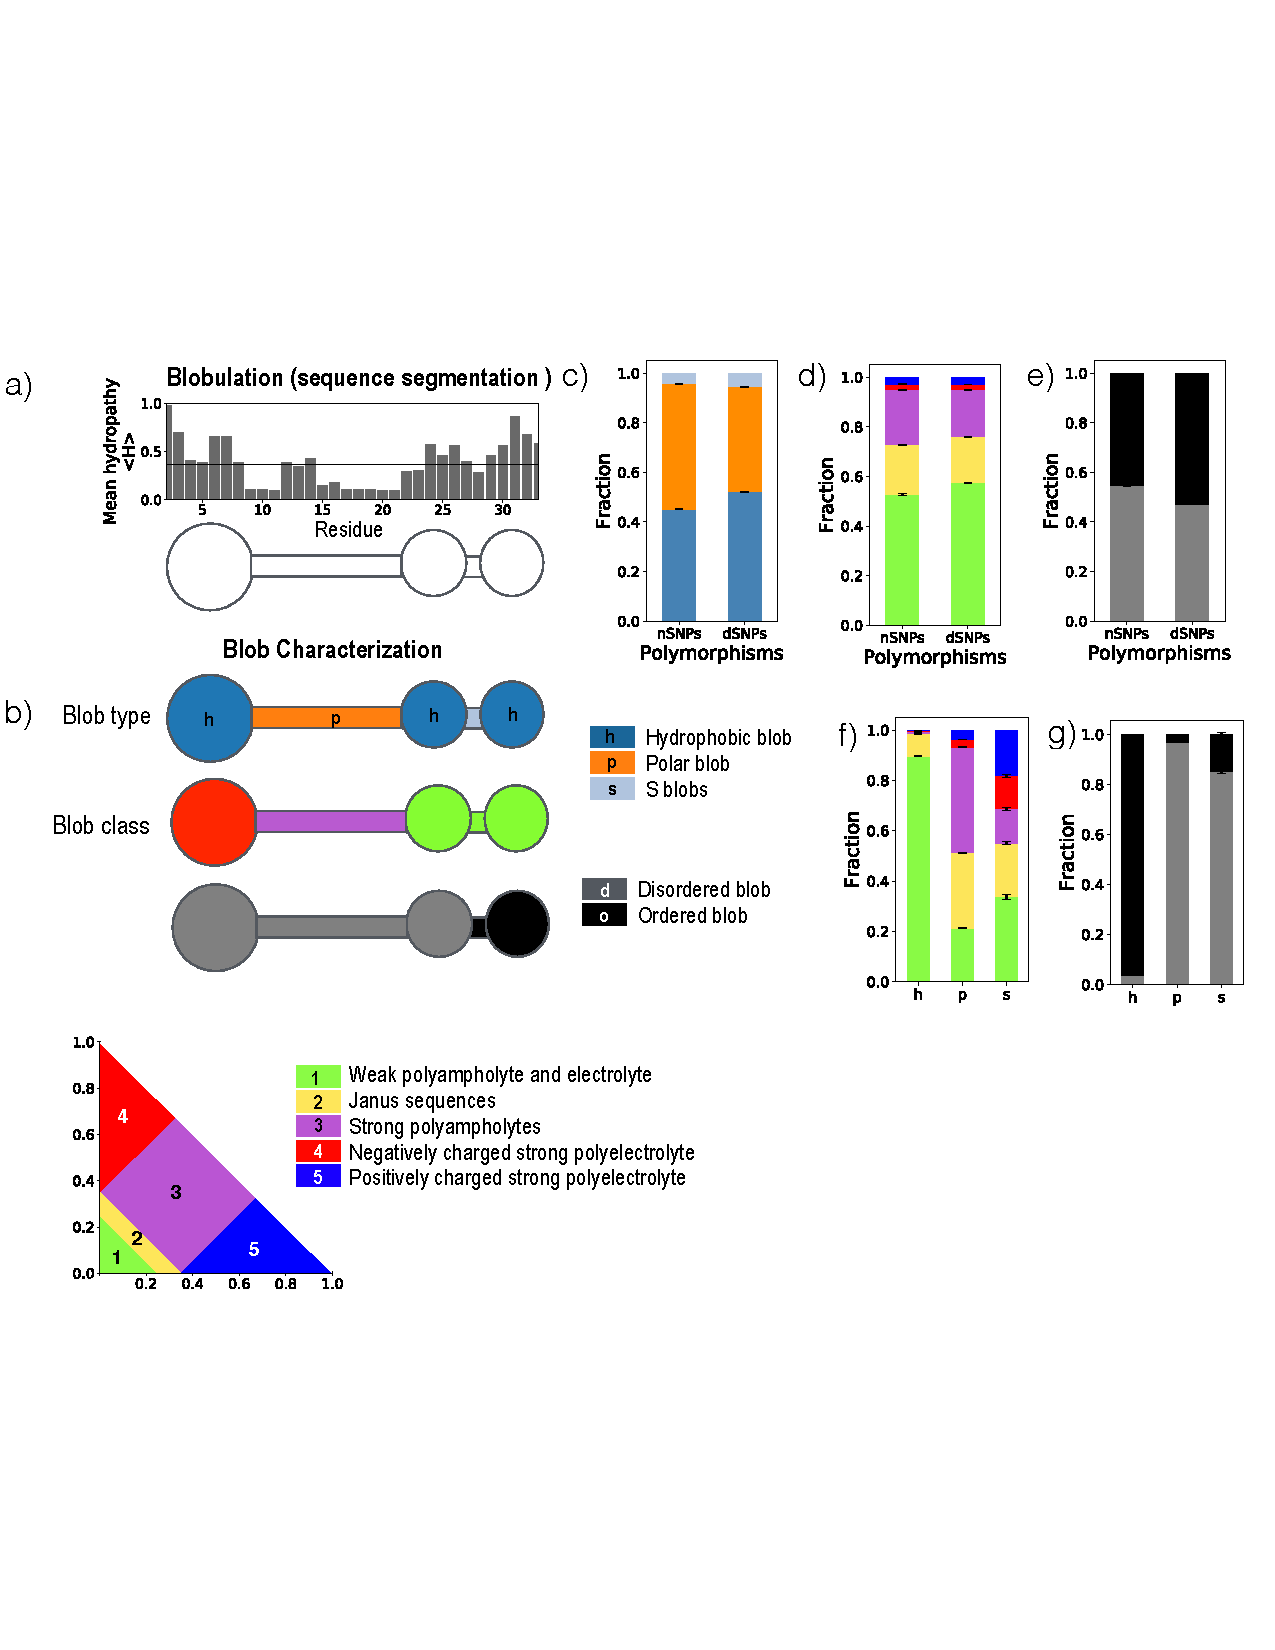
\includegraphics[scale=0.1,width=\textwidth,trim={0 0cm 0 0cm},clip]{./figures/fig1.pdf}
\caption{{\bf Blobulation methodology and distribution of blob characteristics in \dSNPs  and \nSNPs.} a) 
Cartoon representation of the blobulation approach. First,  hydrophobicity (average of 3 residue moving window) is obtained for each residue. Blobs are identified as contiguous stretches of at least 4 residues (unless otherwise noted) in which each residue is above, or each residue is below the hydrophobicity cutoff (black line). \grace{check please, Ruchi} b) Cartoon representation in which the shape of the blobs is determined by \hydrochar: h blobs are shown as circles and p ``blobs" are shown as rectangles. Blobs are colored according to \hydrochar (top) and \chargechar (bottom)  c) Fraction of \nSNPs or \dSNPs that are found in either h blobs (orange) or p blobs (blue). 
d) Fraction of \nSNPs or \dSNPs that are found in blobs of each \chargechar.  (e). Fraction of h or p blobs that are found in each \chargechar.  The distribution in c, d and e are plotted with a cutoff and minimum blob length of 0.4 and 4 respectively. The effect of these parameters on proportion of SNPs in blob type is further discussed in Fig 3b. If enrichment or depletion in \dSNPs is significant (p $< 5\times10^{-3}$) it is annotated with a star.  Errors bars in (c)-(e) represent one standard error for multinomial distributed data.\grace{1. Das Pappu should be its own panel (probably panel b) and should have its own line in the caption. 2. Update blob type and blob class labels. 3. Blue/orange Coloring is still backwards between Panel C and B. 4. Plot in panel e should be before c and d. }  }
\label{c3_h_p_enrich} 
\end{figure}

%\ruchi{The sequence environment local to the SNP often plays an important role in identifying the functional effects of SNPs from sequence. For example SNPs found in evolutionary conserved sequence environment are more likely to be associated with disease than when found in variable sequence environment.}

%We determined the local sequence of a given SNP  by applying the blobulation approach on the entire protein sequence (Fig~\ref{c3_h_p_enrich}a) and then further analyzed the blob containing the SNP. The blobulation was based on residue hydrophobicity with a cutoff of 0.4 along with minimum blob length of 4 (further defined in Methods). 

In order to test blobulation as a meaningful approach for analyzing sequences, we tested whether any blob characterization was correlated with a higher incidence of disease-causing mutations. For each SNP, we applied the blobulation approach on the entire protein sequence (Fig~\ref{c3_h_p_enrich}a) as described in Methods, and then further analyzed the blob containing the SNP. Specifically, we measured the enrichment of disease-associated SNPs (dSNPs) relative to non-disease-associated SNPs (nSNPs) for blobs characterized by \hydrochar{} and \chargechar{} (SNP dataset obtained from Uniprot; see Methods). Unless otherwise noted, \dSNPs are tested for enrichment relative to the expectation set by \nSNPs. For example, the phrase ``\dSNPs are enriched in X blobs" means that \dSNPs are found at a higher rate in blobs of type X than are \nSNPs. Fig~\ref{c3_h_p_enrich}c compares the distribution of blob \hydrochar among \dSNPs and \nSNPs. We find that \dSNPs are enriched in h blobs by about 1.15 fold:  the fraction of \dSNPs in h blobs is (52\%) while the fraction of \nSNPs in h blobs is about 45\%. This is consistent with our previous results from simulations of the long disordered BDNF prodomain, in which h blobs interacted frequently with each other, while p blobs did not form any specific interactions with the rest of the sequence.

In addition to classification by \hydrochar{}, the blobs were also classified according to \chargechar{} (Fig~\ref{c3_h_p_enrich}b), which is the predicted globular phase based on the fraction of positive and negative charges (the Das-Pappu\cite{needed} phase).  
%blob-class (1,2,3,4,5) based on its fraction of charges (Das-Pappu classification). The Das and Pappu phase metrics predicts sequence compactness and is based on fraction of positively (f+) and negatively (f-) charged residues . 
Possible values of the blob \chargechar{} are 1 (Weak polyampholyte), 2 (Janus or boundary region), 3 (Strong polyampholyte), 4 (Negatively-charged strong polyelectrolyte), and 5 (Positively-charged strong polyelectrolyte). Sequences in class 1 have a low fraction of positively charged residues, and nearly all structured proteins fall in class 1. In contrast to structured proteins, IDPs can be found in all five Das-Pappu phases, particularly classes 3, 4, and 5. Therefore the Das-Pappu \chargechar characterization provides a natural metric for distinguishing among sub-categories of IDPs with different functional behavior. 

%These phase metrics are particularly informative for IDPs, as they have higher fraction of charges than structured proteins and are more likely to explore several regions within the metric. 
%\grace{"Explore" isn't quite right, need a better phrase.} 
%Comment- mostly repeated motivation except for the last two sentences
%where strong polyampholytes sequences are likely to have expanded or hairpin conformations, where as weak polyampholytes are likely to have globular conformation. 

The blob \hydrochar{} and \chargechar{} are fundamentally correlated; while blob \chargechar{} does not explicitly consider hydrophobicity, increasing the number of charged residues will reduce the average hydrophobicity of a blob. The extent of this correlation is shown in  (Fig~\ref{c3_h_p_enrich}e), which breaks down the fraction of h and p blobs that fall in each Das-Pappu \chargechar. As expected, most h blobs (89\%) fall in class 1 (weak polyampholyte), followed by 8\% in class 2 (Janus).  The p blobs are more evenly distributed across classes, with the highest fraction (40\%) classified as strong polyelectrolytes.  
%would be equivalent or better than blob \hydrochar{} for stratifying \grace{word choice?} disease-causing and non disease-causing SNPs. %

The distribution of \dSNPs and \nSNPs across blob \chargechar{} are shown in Fig~\ref{c3_h_p_enrich}d. More than half of both \dSNPs and \nSNPs are found in blobs that are weak polyampholytes. \dSNPs are slightly enriched (1.09 fold) for weak polyampholyte blobs.  Due to the high correlation for h blobs and the additional sequence information encapsulated for p blobs, we expected that blob \chargechar{} would be at least as sensitive, if not more sensitive, than blob \hydrochar{} for identifying functional protein segments, and thus have generally higher enrichment for disease-associated SNPs. Surprisingly, we found that the maximum \chargechar{} enrichment (1.09) is slightly less than the enrichment found for h blobs (1.15 fold). Although most hydrophobic blobs are weak polyampholytes, this difference in enrichment suggests that hydrophobicity (rather than simple lack of charge) may be more indicative of sensitivity to mutation.  Strong polyampholytes are depleted among \dSNPs (0.87 fold), which may indicate a relative decrease in blob-blob interactions, since strong polyampholytes tend to be highly solvent exposed. 

%Strong polyelectrolytes are typically solvent-exposed as well, but will also be attracted to blobs of opposite charge.  

%Interestingly, we found that the simpler blob type characterization (based on hydrophobicity) resulted in a higher amount of enrichment than the more complex blob class characterization (based on the fraction of charged residues).   that Blob-type performs slightly better than Blob-class in evaluating the SNPs functional impact (1.15  vs 1.09 fold enrichment).and depleted among strong polyampholyte blobs (0.13 fold).

%\ruchi{The enrichment of \dSNPs in h blobs is not surprising. Several studies have found evidence of correlation between the hydrophobicity of the sequence local to the SNP and its functional impact. SNPs in hydrophobic regions are generally predicted to be buried in protein structure and are found to be more likely to be associated with diseases. It is also consistent with our previous results from BDNF simulations in which h blobs play the role of interaction sites and p blob don’t form any specific interactions with the rest of the sequence.} Comment-should be moved to discussion (our result to their hypothesis comparison) 

\subsection*{Disease-associated SNPs are enriched for mutations that change blob classifications}

\begin{figure}[!ht]
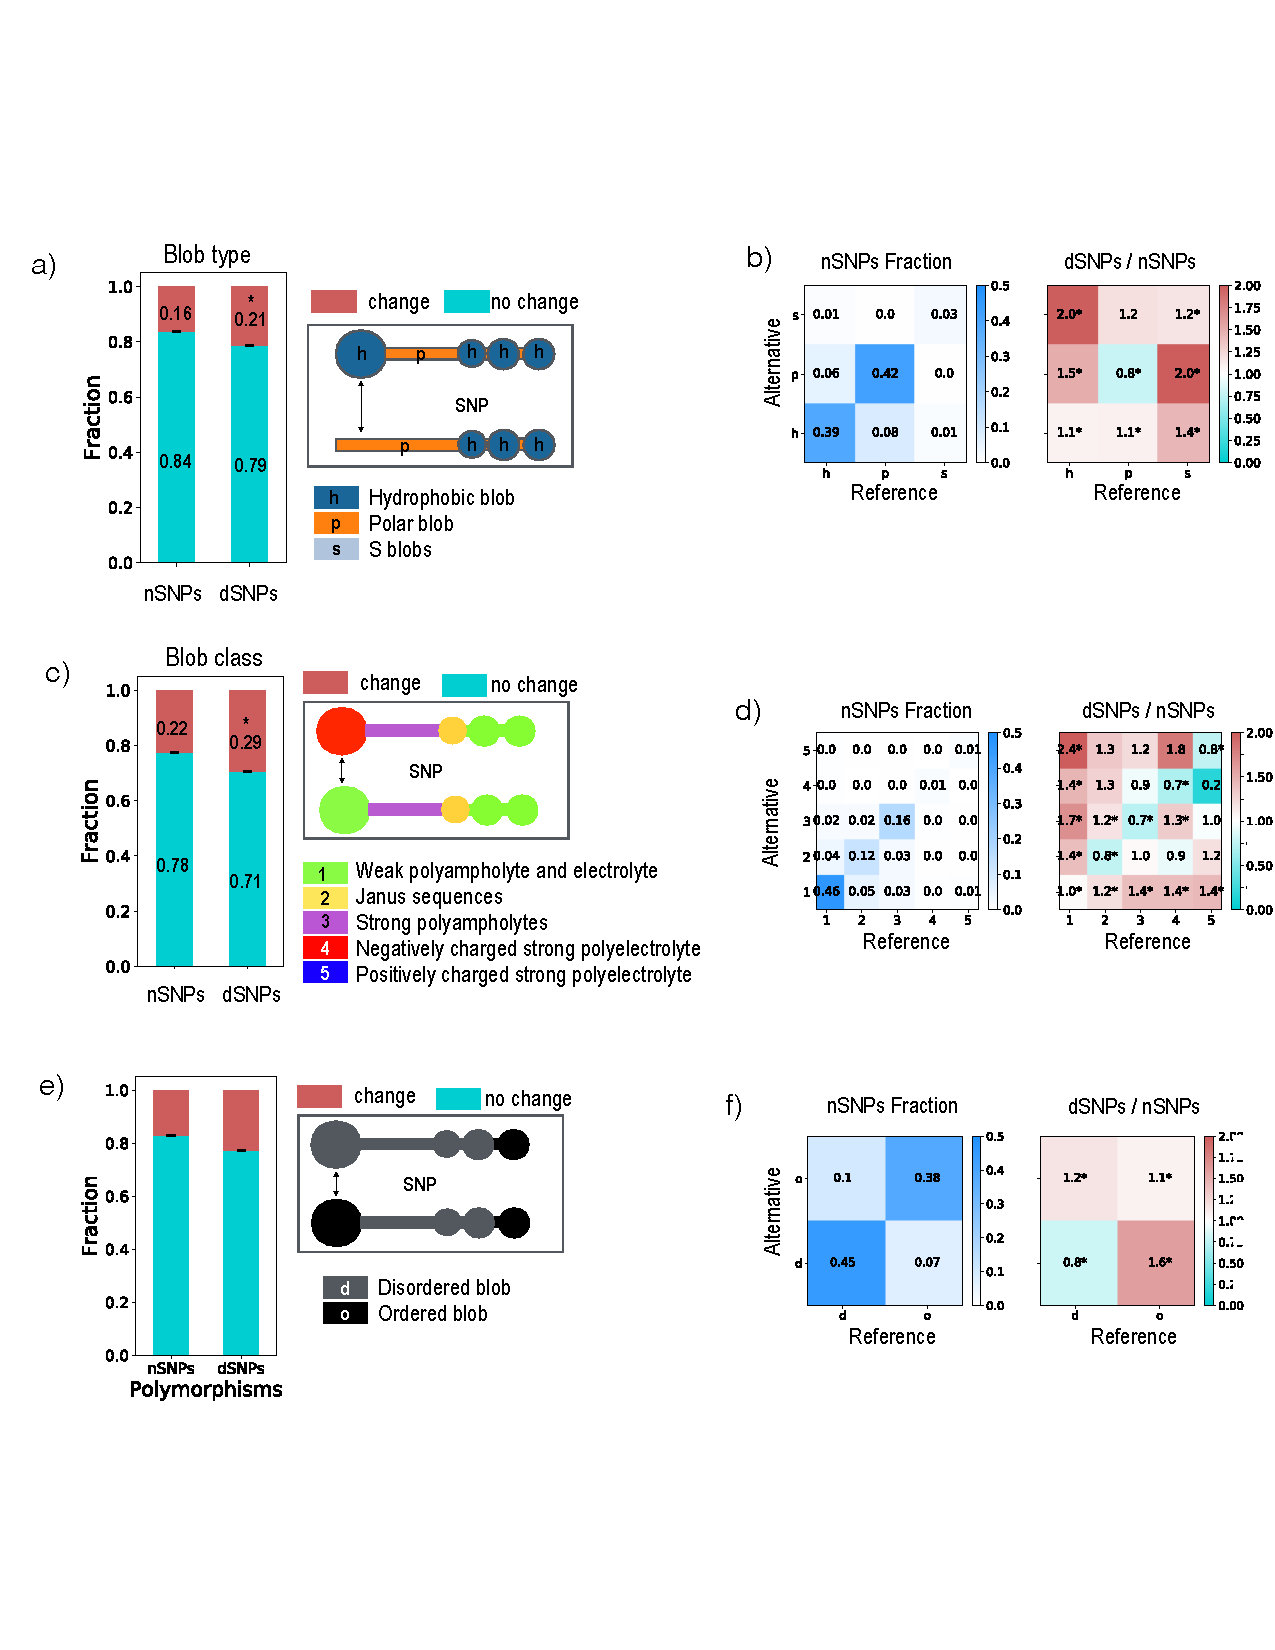
\includegraphics[scale=0.1,width=\textwidth,trim={0 0cm 0 0cm},clip]{./figures/fig2.pdf}
\caption{{\bf Frequency of SNPs that change blob class.} a) Fraction of \nSNPs or \dSNPs that either do (pink) or do not (blue) induce a change in \hydrochar.  b) Fractions (as in a) broken down further by the blob \hydrochar{} before (x axis) and after (y axis) the mutation.  Grid boxes are colored according to the overall fraction of corresponding \nSNPs (left) and the corresponding enrichment ratios (\dSNPs/\nSNPs), with the specific values shown in the boxes. c) As in a, but for transitions in \chargechar. d) As in b, but for transitions in \chargechar.  Fewer than \grace{?} \% of SNPs involve class 4 and 5, and these data are not shown for readability.  For all panels, significant enrichment or depletion in \dSNPs  (p $< 5\times10^{-3}$) is annotated with a star. Errors bars in (a) and (c) represent one standard error for multinomial distributed data.}
\label{blob_transition} 
\end{figure}

Since blob properties like \hydrochar{} and \chargechar{} are dependent upon blob sequence, a SNP may directly result in a change of blob classification. Such transitions will be far more common in shorter blobs, where each residue contributes more to the overall blob assignment. 
%In order to further test the significance of blob characteristics in distinguishing functional variation, we evaluated the enrichment of dSNPs for difference in blob characteristics of original SNP blob and mutated SNP blob. 
%For blob \hydrochar{}, the difference between the original SNP blob and the mutated SNP blob can have two outcomes: (i)  the blob assignment changes; resulting in a h $\rightarrow$ p blob or p $\rightarrow$ h blob ii) the blob assignment does not change; resulting in a h $\rightarrow$ h or p $\rightarrow$ p blob. 
We observe that about 17\% of the \nSNPs and 22\% of \dSNPs involve a blob-\hydrochar{} change, yielding a 1.3 fold enrichment for blob ~\hydrochar{} changes (Fig~\ref{blob_transition}a). 

We calculated the frequency of each of the four possible  blob-\hydrochar{} transitions: h $\rightarrow$ p, h $\rightarrow$ h, p $\rightarrow$ h, and p $\rightarrow$ p (Fig~\ref{blob_transition}b). We find that 7\% of SNPs in the dataset cause h $\rightarrow$ p blob transitions, and these yield the maximum enrichment (1.6 fold) among \dSNPs. These results suggest a particularly high likelihood of functional impact upon introduction of a less hydrophobic residue in a generic hydrophobic sequence (for example, introduction of a charged residue into a buried position).

Slightly more SNPs induce the reverse transition (p $\rightarrow$ h), but \dSNPs have only 1.1 fold enrichment for this transition.  Additionally, SNPs in p blobs causing no blob \hydrochar{} change are depleted among disease-associated SNPs. Overall these results are consistent with the increased mutational sensitivity of hydrophobic (and typically buried) blobs that is shown  in Figure \ref{c3_h_p_enrich}.  

%Previously, in disordered proteins, analogous to blob transitions, disorder $\rightarrow$ order or order $\rightarrow$ disorder transitions due to \dSNPs SNP has been observed~\cite{Vacic2012a, Uversky2014b}.
%
%In structured proteins enrichment or depletion of h blobs could potentially effect the folding core or the kinetics of binding core. 

%It has been found that these transitions frequently disrupt MoRFs in disordered proteins. Because MoRFs mediate protein-protein interactions, it follows that protein interaction networks may also be disrupted~\cite{Uversky2014b}. 

Mutations that reverse residue charge would be expected to have particularly strong functional effects, but would not affect the blob \hydrochar{}. They could, however, affect the blob \chargechar{}. Mutations involving a neutral residue and a charged residue could also directly affect the blob \chargechar{},  either directly, by changing the fraction of positive/negative residues in the original blob or indirectly, by affecting the blob segmentation. \grace{No indirect effect for \hydrochar?} \ruchi{needs discussion}   %or could also the difference between the original SNP blob and mutated SNP blob can have two outcomes (Fig~\ref{blob_transition}c):  (i) it can change the blob \chargechar{} class due to direct or indirect effect a) SNP can directly increase or decrease the fraction of charged residue (FCR) in a blob due to gain or loss of a charged amino acid. This can move the blob into a new region in the Das-Pappu classification ~\cite{Das2013} b) SNP changes the blob \hydrochar{} or blob length, indirectly resulting in a change in blob \chargechar{}. ii) it does not change the blob \chargechar{}, resulting in no change (Fig~\ref{blob_transition}c). 
%We find that about 79\% of the \nSNPs and 70\% of \dSNPs do not cause any blob-\hydrochar{} transition in either \dSNPs and \nSNPs. In line with the above blob-\hydrochar{} observations \dSNPs are 1.3 fold enriched when blob \chargechar{} change is present.
%We further zoomed into the fraction and enrichment in each case of blob \chargechar{} transition 

The frequency of SNP-induced changes in blob \chargechar{} class is shown in Fig~\ref{blob_transition}d, for blobs in category 1 (weak polyampholyte), category 2 (Janus), or category 3 (strong polyampholyte). 
%Frequency and disease enrichment broken down by wildtype blob \hydrochar~ and mutant blob \hydrochar~ are shown in Fig~\ref{blob_transition}d, for blobs in category 1 (weak polyampholyte), category 2 (Janus), or category 3 (strong polyampholyte). 
Transitions involving categories 4 or 5 (positively or negatively-charged strong polyelectrolyte) represented fewer than \grace{how much?} \% of the total transitions. Disease-associated SNPs are enriched for all mutations that change blob \chargechar{} and either unenriched or weakly depleted for mutations that do not change blob \chargechar. The degree of enrichment is largest for transitions between weak and strong polyampholytes, 
%increased with the severity \grace{word choice} of the transition, 
so $1\rightarrow 3> 1 \rightarrow 2$ and $3\rightarrow 1 > 3\rightarrow 2$. Disease-associated SNPs are most strongly enriched (1.8 fold) for SNPS that switch a weak polyampholyte (1) blob to a strong polyampholyte (3) blob were the most strongly enriched for disease-association. This is consistent with evidence that the severity of a SNP on protein function is somewhat \grace{weakly?} correlated with the physicochemical difference between the original amino acid and the missense variant ~\cite{Stone2005}.\grace{Can we make this statement stronger, use more recent reference?}  % $1\rightarrow 3>1\rightarrow 2\sim 3\rightarrow 1 > 2\rightarrow 3\sim 2\rightarrow 1>3\rightarrow 2.   We find that all blob \chargechar{} transitions are enriched. % whereas no transitions either show no enrichment or depletion. This indicates that amino-acid substitution that affect blob \chargechar{} potentially affect protein function. 

These results suggest that transitions in blob ~\chargechar{} may be particularly useful for predicting whether variants have a functional effect.
While generic transitions of blob \hydrochar{} or \chargechar{} yield an equivalent amount of enrichment (1.3 fold) for disease-association, more SNPs in this dataset induce a blob \chargechar{} transition than a \hydrochar{} transition (29\% vs 21\%, respectively). Furthermore, \chargechar{} distinguishes between lower and higher enrichment transitions, since most 1$\rightarrow$ 2 mutations (1.4 fold enrichment) and 1$\rightarrow$ 3 mutations (1.8 fold enrichment) will also count as h$\rightarrow$ p mutations (1.6 fold enrichment). %From this we conclude that for segmentation based on \hydrochar{}, 
This result suggests that for SNPs that change the blob \hydrochar{}, a further split into those with weaker or stronger effects on \chargechar{} provides greater resolution of functional effects. 
%a maximum enrichment observed in blob \chargechar{} is higher than for \hydrochar{} (1.8 fold for 1 $\rightarrow$ 3 vs 1.6 fold for h $\rightarrow$ p).  

%To summarize, we find that difference in Wild Type and SNP blob characteristics is somewhat positively correlated with the functional impact of the SNP. 
%the enrichment between presence and absence of transitions for \dSNPs is very clear, blob class transitions are enriched whereas no transitions either show no enrichment or depletion whereas the same is not true for blob type transitions. 
%\ruchi{There is evidence that the severity of a SNP on protein function is somewhat correlated with the physicochemical difference between the original amino acid and the missense variant ~\cite{Stone2005}. This is in line with previous evidence of correlation between the severity of the SNP and physicochemical difference between original and SNP residue. } comment: move to discussion

\subsection*{Blobulation yields higher enrichment values and more meaningful trends than fixed-length moving windows}

\begin{figure}[!ht]
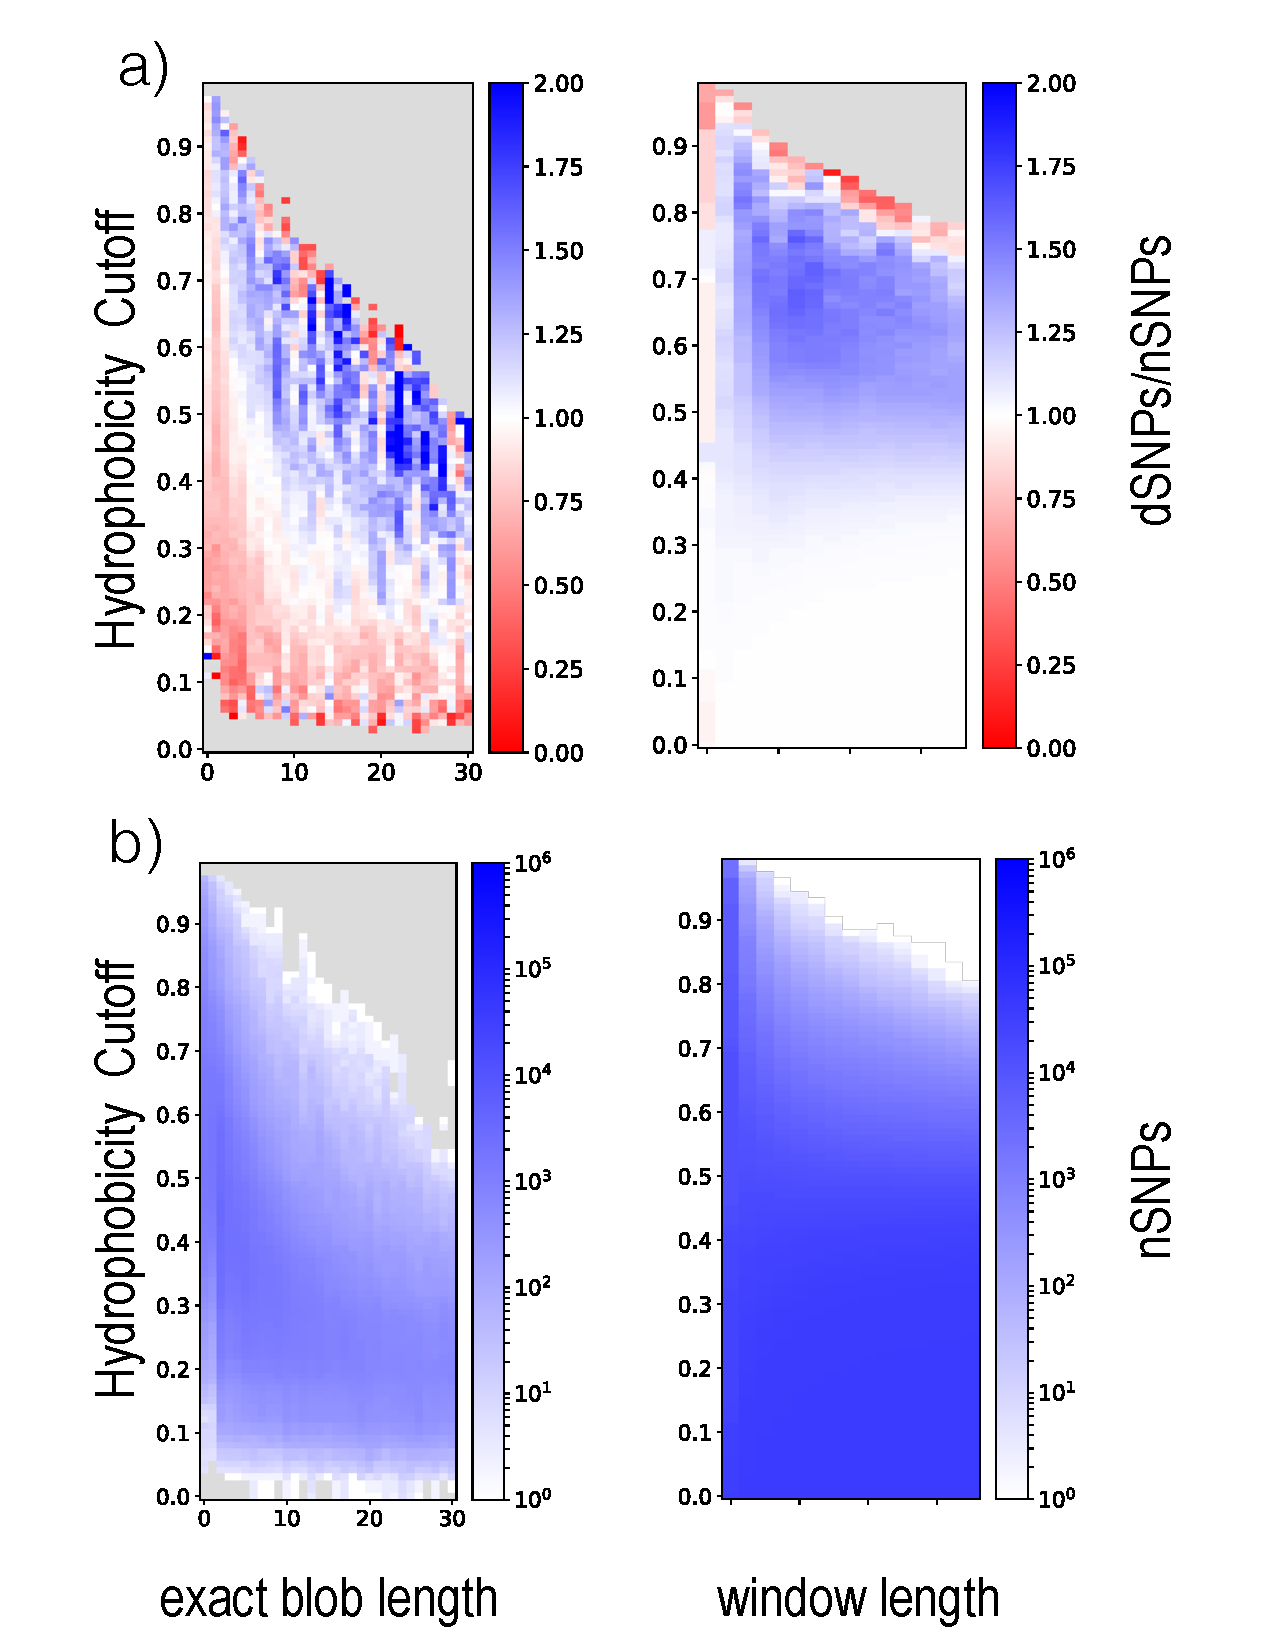
\includegraphics[scale=1,width=0.6\textwidth,trim={0 0cm 0 0cm},clip]{./figures/fig3.pdf}
\caption{{\bf Effect of segmentation approach, length, and hydrophobicity cutoff on calculated enrichment of \dSNPs in hydrophobic segments.} a) 
Enrichment of \dSNPs for hydrophobic segments using a blobulation approach (left) and moving window approach (right).  Blobulation defines a hydrophobic segment (or h blob) as a contiguous stretch of a minimum length in which every residue has hydrophobicity greater than the cutoff.  In contrast, the moving window approach defines a hydrophobic segment as a stretch of residues of a specific length with a mean hydrophobicity that is greater than the cutoff.  \grace{1) Let's discuss non-monotonicity.  Is it real? 2) x axis should be minimum blob length 3) title label is confusing, let's discuss. } Each bin is colored according to the fraction of \dSNPs in hydrophobic segments divided by the analogous \nSNP fraction, with the scale shown in the color bar. No data is shown for parameters in which there are fewer than ten SNPs assigned to hydrophobic segments (gray regions). b) Effect of segmentation parameters on the overall populations of \nSNPs in hydrophobic segments, using the blobulation approach (left) and moving window approach (right). Each bin is colored according to the fraction of \nSNPs that fall in hydrophobic segments.\grace{should show log(fraction).}\matt{i suggest that we make both the x and y bins larger. may alleviate some of the small numbers issues and clean up some of the visible noise. agree that in b) should show log(fraction). And the panels need some form of title/label to show which one is blobulation and which is sliding windows. Also, need to state the bin sizes.}.}
\label{blob_vs_window} 
\end{figure}


The blobulation approach is a particular systematic approach for identifying segments/blobs in the protein sequence. Two parameters (minimum blob length and hydrophobicity cutoff) are required to define blob edges. The degree of enrichment for disease-association is expected to be dependent upon both of these parameters, and we ran the same enrichment tests as in Figure \ref{c3_h_p_enrich} for a wide range of minimum blob lengths and hydrophobicity cutoff values (Fig~\ref{blob_vs_window}a). The highest enrichment is found for blobs that have a contiguous stretch of at least 20 residues with hydrophobicity greater than 0.4; \grace{check values}more than twice as many \dSNPs than \nSNPs are located in such blobs.  \grace{We should provide these as tables in SI} \ruchi{heatmap values?}.
%This continuous trend supports the hypothesis that \hydrochar{} segments constitute identifiable functional elements %and a risk-factor \grace{word choice} for disease-association, and
This result indicates that \hydrochar{}-based sequence segmentation could be particularly useful for assessing the riskiness of SNPs located in long and very hydrophobic sequences.   

%With increasing hydrophobicity cutoff, a non-monotonic trend is observed; the enrichment first increases, reaches a plateau, and then decreases. \grace{Is this decrease real}  This trend is observed regardless of the blob/window length.  

%This was not surprising; it iterates the observation that the higher the local hydrophobicity of a SNP residue, the more likely it is for the SNP to be disease associated. 
%In the above analysis, we defined the local environment of the SNP using blobulation, determining that blob characteristics are indicative of the functional severity of the SNP.  % The significance of the local sequence environment in predicting its functional impact is in fact well explored; nearly all predictors of the SNP's effects exploit this possibility, these predictors define the local sequence environment of the SNP in terms of occurrence of residues inside a window centered on a SNP residue.

In order to compare the effectiveness of blobulation to a moving window approach, we ran analogous enrichment tests for sliding windows across all protein sequences. Two analogous parameters (window length and mean hydrophobicity cutoff) are used for defining hydrophobic regions in the moving window approach, with the resulting enrichment for a range of these values also shown in Fig~\ref{blob_vs_window}a.  Compared to the blobulation approach,  the enrichment detected using the moving window approach is much less sensitive to segment length for windows beyond 6 residues (consider the tilted color bands for the blobulation approach vs the horizontal color bands for moving windows in Figure~\ref{blob_vs_window}a).   

While there is no ``standard" window size, most SNP prediction programs use a window size in the range of 1-21 residues. The window size is chosen to balance concerns that small window sizes may not accurately capture the "local" sequence~\cite{Chen2006, Schlessinger2005, Sander2006} whereas long window sizes can increase signal to noise ratio~\cite{Park2007}. The enrichment insensitivity to window size was thus surprising, but the expected noise was likely lost due to averaging across the proteome.  
As shown in Fig ~\ref{blob_vs_window}b, the overall fraction of hydrophobic segments for mild or moderate hydrophobicity cutoffs was also insensitive to window size, confirming that the dataset we use here is sufficiently large to average out large window noise. For a single SNP, considering too many residues far from the SNP will still contribute significant noise to the prediction.  
%We expect that when the window is expanded by two residues, on average one residue is more hydrophobic and one is less so, and these effects cancel each other when averaged across many sequences. 
%A long moving window would still reduce predictive power of any individual SNP.


Overall, use of the moving window approach yields two-fold enrichment for only a few, scattered parameter values with very few qualifying sequences. 
In contrast, blobulation yielded greater than two-fold enrichment for a well-defined set of parameters (hydrophobicity cutoff $>$ \grace{what?} and minimum blob size $>$ \grace{what?}.  
%This observation supports our hypothesis that an approach like blobulation, which flexibly defines the local sequence based on natural sequence properties, can provide a more powerful approach for predicting disease association than a moving window approach. 
This observation supports our hypothesis that blobulation provides a more meaningful and less noisy approach to protein segmentation than use of a fixed-length moving window.

%More hydrophobic and less hydrophobic regions are indicated by blob \hydrochar{} (h or p, respectively)  for the blobulation approach and by the mean hydrophobicity of residues in the given window length, for moving window approach. Two parameters (minimum blob length and hydrophobicity cutoff) are required to define blob edges. Analogously, two parameters (window length and mean hydrophobicity cutoff) are used for defining hydrophobic regions in moving window approach. For a rigorous comparison, the enrichments were calculated for a wide range of minimum blob length/window length and hydrophobicity cutoff/mean hydrophobicity cutoff (Fig~\ref{blob_vs_window}a).

%For both the approaches, we observe similar trend in enrichment with increase in hydrophobicity cutoff for any given blob/window length. With an increasing in hydrophobicity cutoff, a non-monotonic trend is observed; the enrichment first increases, reaches a plateau, and then decreases. \grace{check on this - is this right?} %This trend is observed regardless of the blob/window length. This was not surprising; it iterates the observation that the higher the local hydrophobicity of a SNP residue, the more likely it is for the SNP to be disease associated. 

%We observe a slightly different trend in enrichment, with an increase in blob/window length for any given hydrophobicity cutoff. The enrichment first increases with increasing blob/window length in cutoff range  0.2-0.6 and 0.4-0.75 for the blobulation approach and moving window approach respectively. Interestingly, the enrichment mostly plateau at large blob length, but decreases at large window lengths ($>$ 21 residues). Moreover, the maximum enrichment observed is higher with the blobulation approach when compared with moving window approach.

%This observation supports our hypothesis that the blobulation approach is likely a better alternative than moving window approach for defining the "local" sequence of a SNP residue. 

%\ruchi{There is no standard window size, and the predictor programs for SNPs use a wide range of window sizes, generally in the range of 1-21 residues. Small window sizes may not accurately capture the "local" sequence~\cite{Chen2006, Schlessinger2005, Sander2006} whereas long window sizes can increase signal to noise ratio~\cite{Park2007}. With the blobulation approach, at a given minimum blob length and hydrophobicity cutoff, the size of the blobs is not constant.} comment - move to discussion

%The logic behind increasing window sizes for better predictions is that one can better account for long-range effects with enlarged windows. However, increase in window size would increase signal to noise ratio. For example even when the SNP is present in charged region, hydrophobic residues far away from the SNP might get picked up. Blobulation approach is less likely to have signal to noise ratio tradeoff, SNP present in charged region will never fall in h blob irrespective of blob length. 

%In order to compare I think the blobulation does more than show higher enrichment -- it is more sensitive to blob length.  I think part of why the moving window curve plateaus is because as you increase the size, you start to pick up hydrophobic regions that are far away from your SNP. There is no need for them to be continuous.

%In the current study, we compare the properties of residues local to the SNP in its sequence for \dSNPs and \nSNPs in humsaver dataset. 
%Fig~\ref{c3_h_p_enrich}a shows the mean hydrophobicity distribution of a SNP's adjacent residue in its sequence for \dSNPs and \nSNPs. We find that in general \dSNPs adjacent residues have slightly higher mean hydrophobicity (0.49) when compared with \nSNPs (0.46).

%To test the hypothesis that the local sequence of \dSNPs has higher hydrophobicity when compared with \nSNPs, we applied our sequence decomposition approach to the sequence associated with each SNP to compare the fraction of SNPs in h blobs in \dSNPs and \nSNPs (Fig~\ref{c3_h_p_enrich}b).  Our hypothesis will be true if \dSNPs is significantly enriched in h blob when compared with \nSNPs 



%We find that about 45\% of the \dSNPs are found in h blobs and the remaining in p blobs (Fig~\ref{c3_h_p_enrich}a). We further compared the enrichment of \dSNPs in h or p blobs. We find that \dSNPs are 1.15 fold enriched in h blobs. 


%The hydrophobic effect is considered to be the major driving force for the folding of globular proteins\cite{Dill1990}. Even though disordered proteins are depleted in hydrophobic residues, it has been frequently observed that small hydrophobic motifs in disordered regions are involved in the binding of these proteins with their partners~\cite{Mohan2006}.  

%The enrichment of \dSNPs in hydrophobic blobs


%To further study the sequence properties of \dSNPs and \nSNPs, we further assign each blob a class (1,2,3,4 or 5) depending on the Das and Pappu metrics (Fig~\ref{c3_h_p_enrich}d). 

%Fig~\ref{c3_h_p_enrich}e shows the fraction of SNPs falling in each class for \dSNPs and \nSNPs. For both \dSNPs and \dSNPs $>$50\% of SNPs fall in weak polyampholyte blob. However, \nSNPs are enriched (1.09 fold) in weak polyampholyte blob whereas \nSNPs are enriched in strong polyampholyte blobs. 

%To understand the relationship between blob class and blob type, we further looked at the distribution of each blob class for a given blob type (Fig~\ref{c3_h_p_enrich}f). We find that h blobs are likely weak polyampholyte whereas p blobs are distributed among each class type with about 40\% as strong polyelectrolyte. 

%To summarize, we find that \dSNPs are enriched in h blobs type or weak polyampholyte class. 
%This is consistent with the observation that disease-associated SNPs are depleted in long linker regions probably because they do not form any specific contacts with the rest of the sequence.
%It has been shown that hydrophobicity score of \begin{equation}\frac{H_{i}+H_{i-1}+H_{i+1} }{3}\label{eq:bond}\end{equation}



%We find that \dSNPs frequently transitions a strong polyampholyte blob to weak polyampholyte blob and vice versa in both ordered and disordered SNPs. 

%We find that more than 25\% of \dSNPs can change phase annotation. The phase annotation and $\kappa$ values predict if a blob is collapsed and e\timespanded ~\cite{Das2013}. 
%It has been frequently observed that PTMs such as Ser/Thr phosphorylation can change the FCR and NCPR properties of IDPs and can thus tune the sequence ensemble relationships of IDPs due to their polyampholytic nature~\cite{Firman2018, Das2013}. 
%We further examined the specific phase annotation transitions observed (Fig~\ref{c3_pappu_enrich}). 



%\subsection*{Comparing \dSNPs and \nSNPs blob types in aggregating proteins}
\subsection*{Disease-causing SNPs in aggregating proteins are particularly enriched in hydrophobic blobs}

\begin{figure}[!ht]
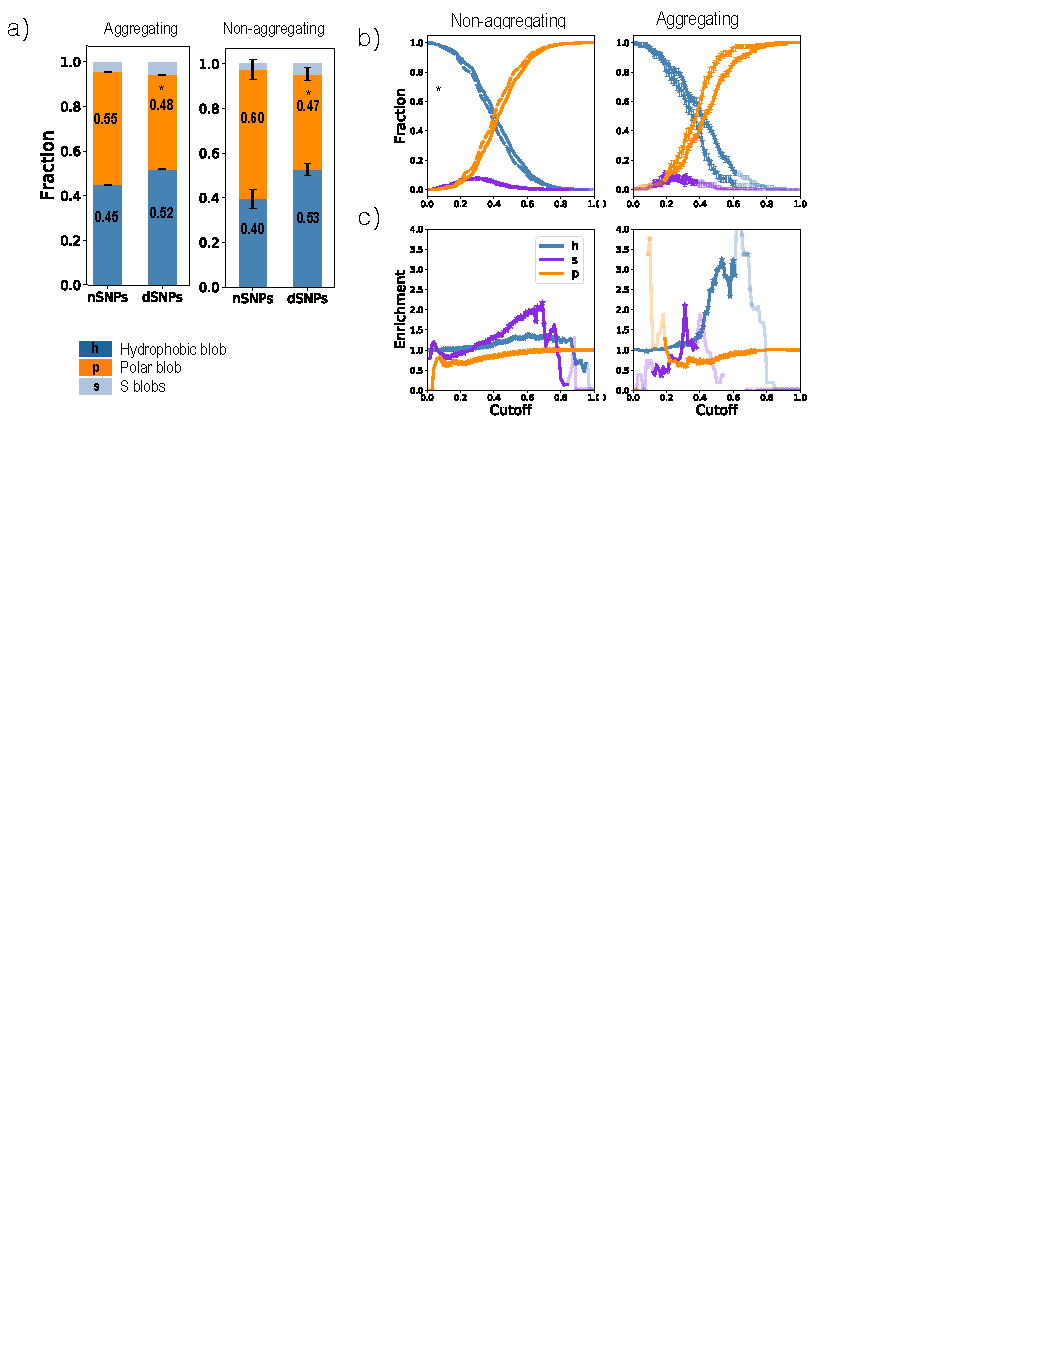
\includegraphics[scale=0.1,width=\textwidth,trim={0 0cm 0 0cm},clip]{./figures/fig4.pdf}
\caption{{\bf Blob hydrophobicity for SNPs in aggregating proteins.} a) Fraction of SNPs that fall in h or p blobs in known-aggregating proteins (left) and all others in the dataset (right). b) The population of \nSNPs (dashed) and \dSNPs (solid) in h (blue) or p (orange) blobs for a given hydrophobicity cutoff, in known-aggregating proteins (left) and all others (right).  \dSNPs are significantly enriched in hydrophobic blobs for both aggregating and non-aggregating proteins (p $< 5\times10^{-3}$, indicated by a star). Error bars represent one standard error for multinomial distributed data. c) The corresponding enrichment (\dSNP fractions divided by  \nSNP fractions) for a range of hydrophobicity cutoffs.   All blob assignments used a minimum blob length of 4, so the values for non-aggregating proteins are equivalent to the x = 4 column in the left heat map of Figure \ref{blob_vs_window}A.  
%If enrichment or depletion in \dSNPs is significant  it is annotated with a star. 
 }
\label{agg_enrich} 
\end{figure}

%\begin{figure}[!ht]
%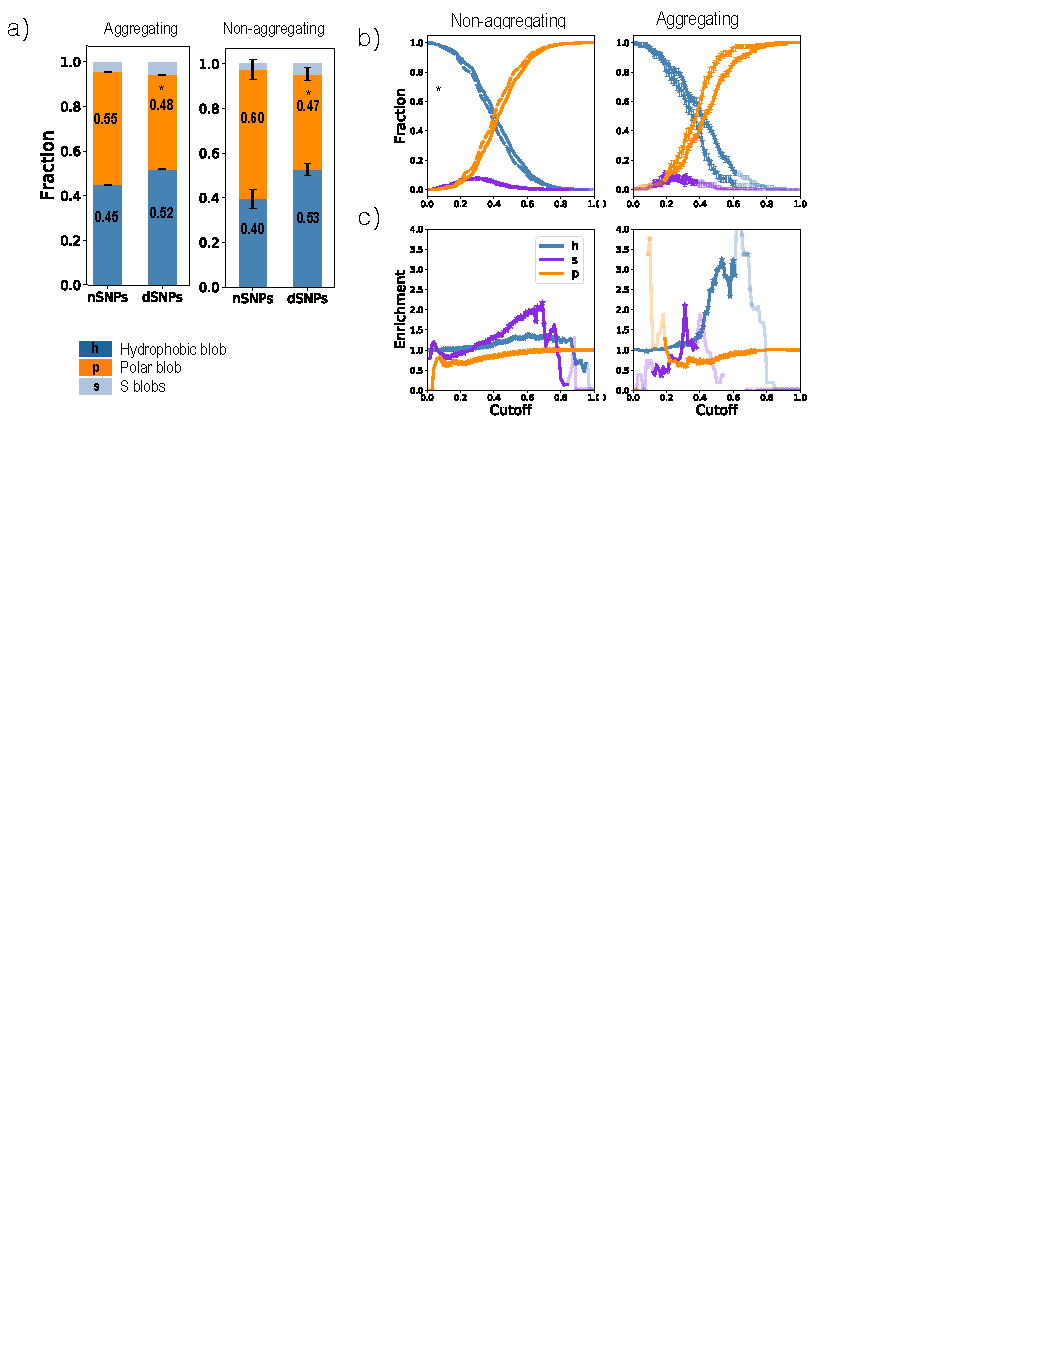
\includegraphics[scale=0.1,width=\textwidth,trim={0 0cm 0 0cm},clip]{./figures/fig4.pdf}
%\caption{{\bf Polyphen-2 prediction for Aggregating proteins and Non-aggregating proteins dataset} a) Population of benign,  possibly damaging and probably damaging SNPs predicted in \dSNPs and \nSNPs for Aggregating proteins and Non-aggregating proteins. b) The sensitivity of Pholyphen-2 for \dSNPs dataset found in h blobs for aggregating and non-aggregating proteins.}
%\label{polyphen} 
%\end{figure}

In order to test the hypothesis that the blob \hydrochar is a stronger predictor of the functional impact of a SNP in aggregating proteins when compared to non-aggregating proteins, we separated known aggregating proteins out of the dataset. Proteins involved in formation of extracellular amyloid deposits or intracellular inclusions with amyloid-like characteristics are labelled as "Aggregating proteins" (28 proteins, 124 nSNPs, 330 dSNPs) and all the remaining proteins are labelled as "Non-aggregating proteins". 

As shown in Fig~\ref{agg_enrich}a, with the mild hydrophobicity cutoff of 0.4 used in Figs(\ref{c3_h_p_enrich} and \ref{blob_transition}), \dSNPs in aggregating proteins have a 1.33 fold enrichment in h blobs. In comparison, \dSNPs in non-aggregating proteins show a 1.15 fold enrichment in h blobs. This is consistent with the well-established hydrophobicity of aggregating proteins, including the hydrophobicity of amyloidogenic sequences\cite{Tzotzos2010,Abskharon2019}, and further supports the hydrophobic regions of those proteins as particularly sensitive to mutation. \grace{Need a sentence comparing to hot spot detection, particularly whether residues with high hydrophobicity also have high aggregation tendencies. Sentences in the blue paragraph just below are too vague for this section, but circle around what we need.}  

\ruchi{Among various sequence properties identified as aggregation characteristics (hydrophobicity, charge, alternating patterns of hydrophobic and hydrophilic stretches, secondary structure propensity, packing density), residue hydrophobicity has been fairly common. Aggregation ``hot spots" are often found in the hydrophobic core of the proteins.  Since, hydrophobicity is one of the few residue properties used for identifying aggregation ``hot spots", it will likely be a stronger determinant for the functional impact of SNPs in theses proteins when compared with the functional impact of SNPs in non-aggregating proteins. Finding SNPs in aggregation ``hot spots" is similar to finding SNPs in the functional/active sites of proteins, since these SNPs can directly affect the proteins' aggregation propensity and function. comment repeated motivation } 

More significantly, the enrichment for \dSNPs in the h blobs of aggregating proteins increases steadily as the requirements for h blobs are made stricter, reaching a maximum of 3 fold \grace{exact number?} enrichment for blobs meeting a 0.6 hydrophobicity cutoff (Fig~\ref{agg_enrich}b).   This is consistent with previous observations that the in vitro aggregation rate of unstructured polypeptide chains is proportional to hydrophobicity and inversely proportional to net charge\cite{DuBay2004}.  In contrast, non-aggregating proteins are relatively insensitive to hydrophobic cutoff, reaching a maximum enrichment of less than 1.5 fold.  

%The success of the tested hypothesis highlights the wide applicability of the blobulation approach for identifying segments within a protein sequence.

%The high enrichment of \dSNPs in h blobs is very consistent with previous observations, including the hydrophobicity of amyloidogenic sequences \cite{Tzotzos2010,Abskharon2019}.  More directly, the in vitro aggregation rate of unstructured polypeptide chain is proportional to hydrophobicity and inversely proportional to net charge\cite{DuBay2004}.  


%However, our study provides the first evidence of the pathogenic fate of a mutation when found in h blobs of aggregating proteins from genomics data-set. 

%We further tested if the high enrichment observed in h blobs for Aggregating proteins can be predicted by commonly used mutation predictor such as PolyPhen-2. We find that PolyPhen-2 is less efficient for Aggregating proteins (Sensitivity:60\%, Specificity:49\%) when compared to aggregating proteins (Sensitivity:80\%, Specificity:60\%)(Fig~\ref{polyphen}a). To further test the sensitivity of PolyPhen-2 to h blobs, we measured the sensitivity of PolyPhen-2 within h blobs for Aggregating and Non-Aggregating proteins (Fig~\ref{polyphen}b). We find that any increase in h blobs hydrophobicity threshold does not cause any significant increase in the sensitivity of PolyPhen-2. 

%We find that PolyPhen-2 does not work very well for Aggregating proteins. This was not surprising, especially given that most Aggregating proteins are IDPs or contain large number of IDRs. Vacic et al\cite{Vacic2012a} showed that mutation predictors such as PolyPhen-2 and SIFT does not work well for IDPs. Notably, the SNPs dataset investigated here overlaps with the predictors’ training sets, and the reported accuracies are likely to be lower when applied to out-of-training set examples. Our finding underscore the significance of h blobs which is not present in predictive disease mutation models such as PolyPhen-2. Recently, Abskharon et al\cite{Abskharon2019} used \times-ray crystallography and found the critical role of hydrophobic regions in Prion protein misfolding. 


%We grouped 25 proteins and all its 379 SNPs (281 \dSNPs and 98 \nSNPs) from our dataset and analyzed them separately for enrichment in h and p blobs. This further indicates that h blobs are interaction sites for these aggregation-prone proteins. 

%\begin{figure}[!ht]
%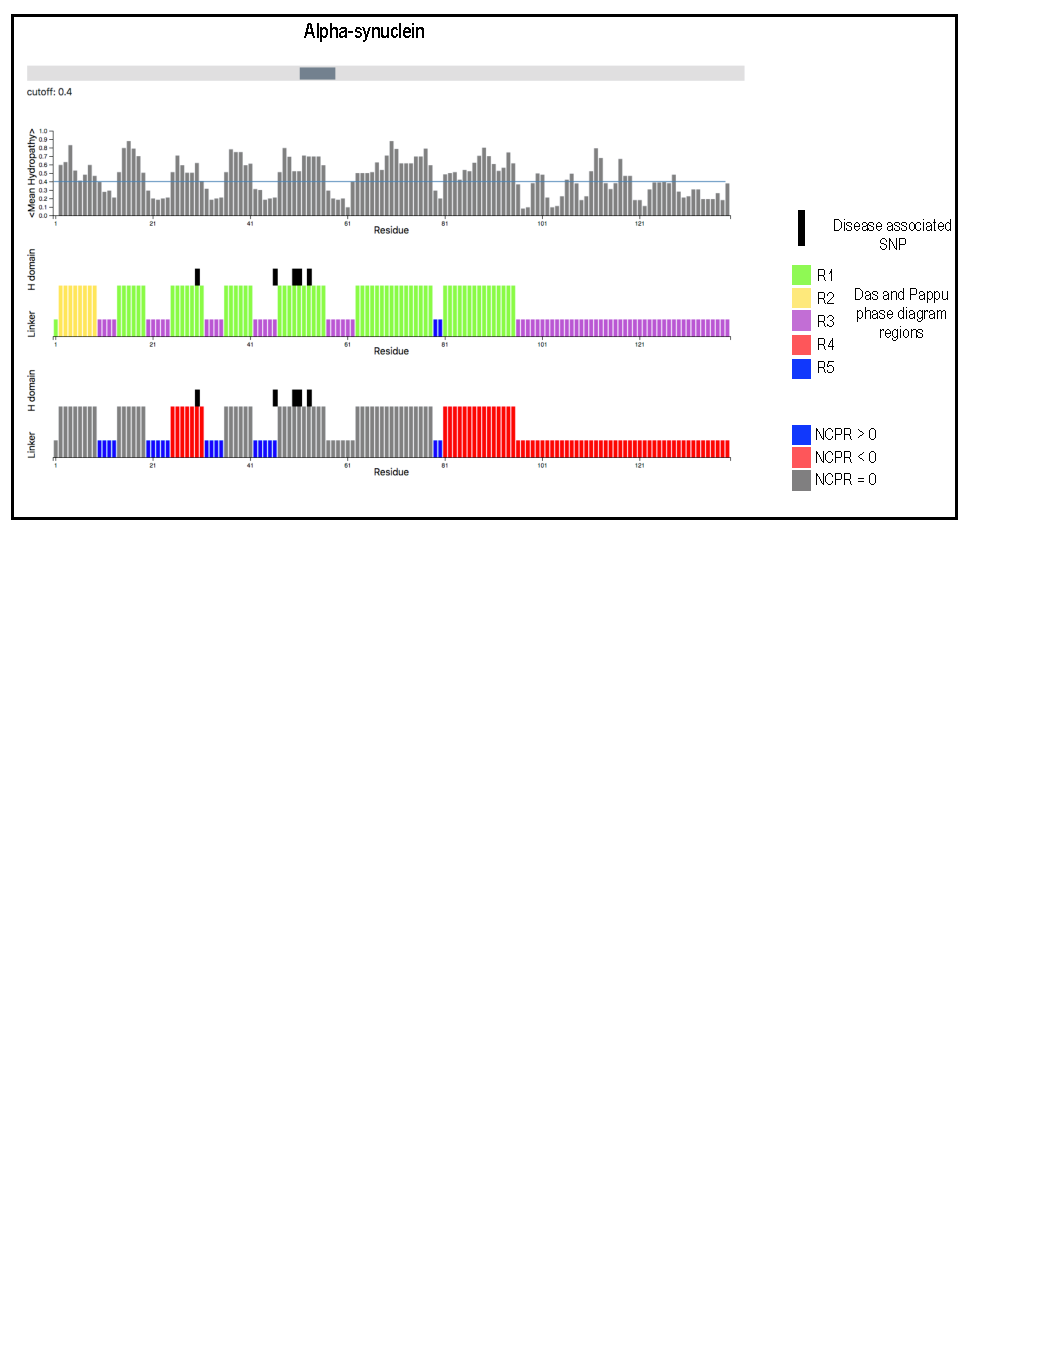
\includegraphics[scale=0.1,width=\textwidth,trim={0 0cm 0 0cm},clip]{./figures/c3_tool_eg1.pdf}
%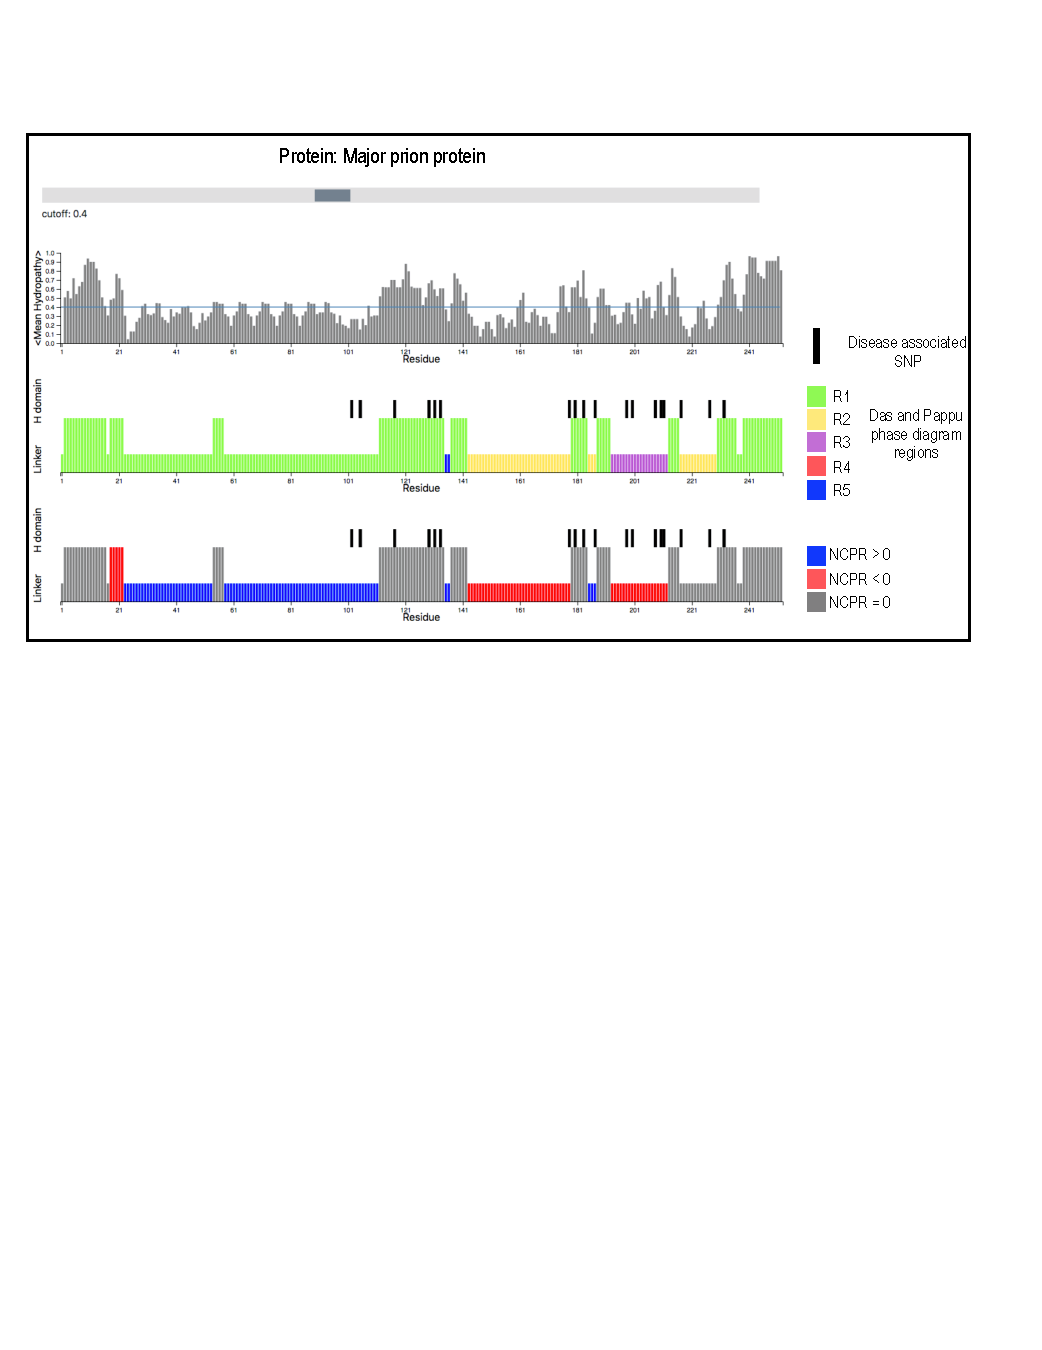
\includegraphics[scale=0.1,width=\textwidth,trim={0 0cm 0 0cm},clip]{./figures/c3_tool_eg2.pdf}
%\caption[\bf Example of sequence decomposition approach applied to disordered proteins using the web tool.]{{\bf Example of sequence decomposition approach applied to disordered proteins using the web tool.} Sequence decomposition approach applied to $\alpha$-synuclein (top) and major prion protein identified by (bottom). The first row shows the mean hydrophobicity per residue (top), the middle row shows the digitized hydrophobicity colored by phase diagram region, and the bottom row is colored by net charge per residue. Within the digitized hydrophobicity, the high regions correspond to hydrophobic blobs, while the low regions correspond to non-hydrophobic blobs. \dSNPs SNP location is annotated with black bars}
%\label{tool_snapshot} 
%\end{figure}

%Conceptualization of long structured proteins relies heavily on the consecutive secondary structure elements that form the protein's topology, allowing for a coarse cartoon-style representation. No such approach for constructing an IDP topology has been available. In the current work we have also identified sequence properties of IDPs that are informative for whether mutations are likely to impact function. We have created a web application tool that visualizes this information for user-input protein sequences.

%We thus present this conceptual tool, that will allow others to easily impose this sequence representation for their protein of choice and visualize the location of disease-associated SNPs within this representation (Fig~\ref{tool_snapshot}). It also lets the user visualize the blobs at any cutoff in the range of 0-1. 

%\subsection*{Examining the identified blob properties in BDNF prodomain simulations}
\section*{Discussion}

In the present work, we have tested whether the protein ``blobulation" approach we developed in \cite{Lohia2019} for a specific disordered protein is a meaningful approach for identifying segments across generic proteins.  We found that 
\begin{enumerate} 
\item Overall, disease-associated mutations are weakly enriched (1.15 fold) in hydrophobic blobs. 
\item Disease-associated mutations are moderately enriched for mutations that cause transitions in blob~\hydrochar{} (up to 1.6 fold) and strongly enriched for mutations that cause certain transitions in blob~\chargechar{} (1.8 fold).
\item Enrichment of disease-associated mutations in hydrophobic blobs increases with the strictness of the hydrophobic blob criteria.  
\item SNPs in variable-length hydrophobic blobs were more strongly associated with disease than SNPs in fixed-length hydrophobic moving windows, regardless of the parameters used. 
\item Disease-causing SNPs in aggregating proteins were particularly enriched in hydrophobic blobs. Disease-associated SNPS were more than 3 fold enriched in h blobs that met the strictest criteria. 
\end{enumerate}
These results support the use of blobulation as a simple method for segmenting proteins, requiring only the protein amino acid sequence and two parameters (minimum blob length and hydrophobicity cutoff). Once blobs are identified, they can be characterized on any property of interest, including  mean hydrophobicity, net charge per residue, fraction of polar residues, fraction of disordered residues, etc. The present results also support a role for hydrophobicity in determining the sensitivity of a given protein region to disease-causing mutations. 

%These segments (also referred to as blobs) define the 'local sequence' for a residue more effectively than the moving window approach most commonly used in sequence-only methods.  Blobulation is a simple method requires only the protein's primary sequence, along with two parameters of minimum blob length and cutoff. Once the blobs are identified, they can be characterized on any property of interest such as mean hydrophobicity, net charge per residue, fraction of polar residues, etc. Blobulation and blob characterization are especially meaningful for long protein sequences. The average property of a long protein is insensitive to a single residue change. However, the identified blobs are more likely to be sensitive to this change. 

We anticipate that these results may further efforts to assess functional significance of SNPs for which disease-causality is uncertain.  Despite the wealth of genetics information presently available, %(gnomAD~\cite{Karczewski2019},OMIM~\cite{McKusick2007},ClinVar~\cite{Landrum2018}), 
the complex nature of many phenotypes makes the identification of causal variants difficult~\cite{Claussnitzer2020}. Widely used methods to find genotype/phenotype associations, such as pedigree-based linkage studies or population-based association studies, have identified thousands of associations with a wide spectrum of phenotypes and diseases~\cite{Buniello2019, Gallagher2018, Tam2019}. Association of a SNP with a disease does not necessarily indicate  causality, ~\cite{Boyle2017, Goldstein2009, McClellan2010,MacArthur2014}  %For example, alleles that happen to be in strong linkage disequilibrium with causal variants will also show statistical association. Other lines of evidence are often needed to identify or prioritize likely functional variants, 
motivating the development multiple complementary approaches for predicting the functional effects of SNPs. 

%Systematic experimental methods, such as electrophoretic mobility shift assays (EMSA) or CRISPR/Cas9-based gene editing technology, can isolate casual variants, but the time-consuming and expensive nature of these assays makes them unfeasible to apply on such large volume of variants~\cite{Soldner2016, Liu2017} . In the past two decades, various high-throughput bioinformatics tools for analyzing variants at the DNA, RNA, and protein level have become available~\cite{Webster2019}. Despite the availability of large number of these methods (more than hundred in silico variant effect predicting methods are available at protein level ~\cite{Hu2019}), their clinically relevant prediction accuracy remains elusive. The first problem with clinical application is choosing the suitable tool, which is primarily challenging due to difficulty in performance comparison. Although there are some benchmark studies available~\cite{Niroula2018}, the performance varies widely, for example, due to sizes of the dataset used for comparison~\cite{Grimm2015, Riera2016, ValeFerreira2019, Frousios2013,Schiemann2016}. 

%Most state-of-the-art SNP prediction methods rely (either directly or indirectly) on sequence homology across multiple proteins\cite{Thomas2004, Ng2001, Stone2005}. This approach is effective when it is applicable, such as mutations found in evolutionary conserved functional proteins~\cite{He2018}. However, not all functional variation is in highly conserved regions. For example, intrinsically disordered proteins (IDPs), which are proteins that lack unique structure in at least one of their functional forms, are involved in critical biological functions~\cite {Uversky2013a,Panchenko2015,Ward2004a,Dyson2005a,Uversky2019} and evolve rapidly (are typically poorly conserved across species~\cite{Brown2011}).  Moreover, protein regions that have low sequence conservation are intrinsically likely to include a large number of SNPs. Many SNPs in IDPs contribute to common population variation, and many have been associated with signaling~\cite{Uverskya,Deiana2016} and aggregation disorders~\cite{Patel2015,Uversky2015}, including psychiatric\cite{needed}, neurodegenerative~\cite{Weinreb1996}, and aging-related decline~\cite{CuanaloContreras2013}. Genes with importance for drug absorption, distribution, metabolism, and excretion (ADME) are also highly variable~\cite{Gaedigk2016, Fujikura2015, Colledge2012}. Predicting the functional impact of SNPs in evolutionary variable sequences such as IDPs is an active area of research ~\cite{Vacic2012a,Ali2014}due to lack of effectiveness of popular sequence homology based methods.

%The mechanisms underlying SNP causality are often established using in vitro experiments, although evolutionary methods reflect the in vivo effects of a mutation. but. In principle, computational methods can predict in vitro effects of a mutation in any single protein sequence, including de novo sequences, and multiple efficient methods have been developed with that goal in mind. Bioinformatics approaches apply known principles of protein physical chemistry to the local sequence, in order to consider the effects of the mutation on properties like the residue mass, size, charge, hydrophobicity, C-beta density, and residue flexibility~\cite{Hecht2015, needed}.  Such methods may also rely on known protein structures in order to incorporate properties such as local secondary structure and solvent accessibility. In the absence of structural information, however, computational prediction accuracy is low, and full three-dimensional structures have been experimentally solved for a tiny fraction of proteins~\cite{Mir2017,Rose2016}. With few exceptions, therefore, these methods have not been applied on a genome-wide scale.  

All protein level methods rely on some form of residue characterization for such predictions. In addition to physicochemical properties~\cite{Stone2005, Niroula2015, LopezFerrando2017,Hecht2015,Popov2019} similar to the \hydrochar{} and \chargechar{} considered in the present work, these may include evolutionary conservation~\cite{Stone2005, Thomas2004, Ng2001, Choi2012, Hecht2015, Niroula2015,Thomas2004,Capriotti2006} and structural propensities~\cite{Iqbal2019, Ittisoponpisan2019, Capriotti2004,Capriotti2005, Parthiban2006, Wainreb2010,Popov2019}. Methods relying on physiochemical properties are uniquely suited for application to disordered sequences and weakly conserved sequences, and may be compared directly against in vitro experimental results for mechanistic consistency. Yet many are still limited by a reliance on structural information for predictive accuracy.  

While structural data implicitly provides insight into the segmentation of a protein sequence, we show here that segmentation may be meaningfully estimated from the sequence alone. Based on the present results, we suggest that structureless methods may recapture some accuracy of structure-based methods by introducing sequence-based segmentation.  While we propose blobulation as a simple approach for doing so, in principle, secondary structure prediction could be used instead. For many proteins, however, this approach would be frequently unfeasible and overly restrictive. In addition to the challenges inherent in predicting secondary structure (which may be highly sensitive to the local protein environment or simply non-existent), many secondary structure prediction methods require alignment to a homologous sequence with known structure. ~\cite{Yang2018, Zhang2018a,Wang2017,Aydin,Ma2018}. This is essential for secondary structure predictors to achieve their primary goal: distinguishing \textit{between} secondary structures. Segmentation, however, only requires knowing where the segment begins and ends.  



%Bioinformatics methods for predicting SNP causality based on physicochemical properties frequently rely on known protein structures; in the absence of structural information, computational prediction accuracy is low. Among other information, structural data implicitly provides insight into the segmentation of a protein sequence.  Unfortunately, full three-dimensional structures have been experimentally solved for a tiny fraction of proteins~\cite{Mir2017,Rose2016}. \grace{less than half? less than 10 percent? less than 1 percent? human proteins or all proteins? } %Nonsynonymous SNPs change the side-chain of a given amino acid, which may certainly perturb intramolecular interactions, shifting the backbone conformation (i.e. the “structure”). 
%and functional effects are ultimately determined by changes to intermolecular interactions, including interactions of the protein with solvent, ions, ligands, or other proteins. Changes to intermolecular interactions may be induced by changes in structure but do not require them. %As an example, the pentameric ligand-gated ion channel family is highly structurally conserved, but sequence variations allow some channels to conduct cations while others conduct anions. The functional implications are substantial: anionic channels inhibit neurons while the cationic channels excite them. The protein-ion interactions differ, but the protein structure does not. We therefore focus on properties of a sequence that are likely to affect intermolecular interactions.  

SNP-prediction methods often test residue properties for relevance by machine learning algorithms such as neural networks~\cite{Bromberg2007, Hecht2015, LopezFerrando2017}, Hidden Markov Models~\cite{Thomas2004,Shihab2012}, Random forests~\cite{Niroula2015, Wainreb2010} or Support vector Machines~\cite{Yue2005,Rentzsch2018,Calabrese2009,Capriotti2006}). The machine learning methods derive their decision rules based on training datasets of annotated mutations, and therefore are sensitive to the training set used. Machine learning methods also rely on a large number of features, which can obscure the biological relevance of any given feature. Here we have instead performed hypothesis-driven tests for enrichment of certain features in putatively causal SNPs, based on the principle that those features that are most relevant for evaluating SNPs should be detectable by simple enrichment tests. Nonetheless, the characteristics of the SNP-containing blob should be straightforward to add as an input to a machine-learning model. In particular, it could be a tractable approach for combining blob-level information with protein-level information, as we did for the particular case of aggregating proteins. 


%Among the two blob characteristic we examined for SNP enrichment, we find that h blobs are a bet



%Historically,  a form of blobulation approach has been used for identyfying transmembrane helix region from protein sequence. And has also been used for identifying solvent exposed residues and disordered regions. 


% single-sequence based approach and can be easily applied to de novo sequences as well. 




%It has been frequently observed that PTMs such as Ser/Thr phosphorylation can change the FCR and NCPR properties of IDPs and can thus tune the sequence ensemble relationships of IDPs due to their polyampholytic nature~\cite{Firman2018, Das2013}. 

%We show that blob hydrophobic character (blob-type) 
%Pathogenic transformations of IDPs are also often triggered by altered PTMs. 



%demonstrate the application of using blobulation approach for identifying segments within proteins. 

%shows that \dSNPs frequently 1) are enriched in h blobs. This effect is even more pronounced for aggregation related proteins, 2) causes blob transitions; h to p or p to h transitions, 3) causes phase annotations transitions; could change the blob to stronger or weaker polyampholytes, 3) occur in h blobs and the frequency further increases as the length of the blob increases 4) are depleted in p blobs but the depletion decreases as the length of the blob decreases. 

%The current phase diagram of IDPs are insensitive to single residue substitutions for long proteins. For example in an IDP of more than 30 residues, a single charge addition or deletion would probably not change the predicted phase behavior, because the number of changed residues is very small compared to the total number of residues. Firman et al~\cite{Firman2018} showed that the certain regions within the Das and Pappu classification are more sensitive to very small changes in FCR. With our current sequence decomposition, identified blobs are much more sensitive to a single residue mutation including charge neutral mutations.
%Blob transition will be more sensitive to PTMs, secodanry structure elements. Transmembrane regions

%It has been frequently observed that PTMs such as Ser/Thr phosphorylation can change the FCR and NCPR properties of IDPs and can thus tune the sequence ensemble relationships of IDPs due to their polyampholytic nature~\cite{Firman2018, Das2013}. 

%In structured proteins, enrichment or depletion of disease mutations in h blobs can disrupt the folding core or the kinetics of the binding core as well as specific interactions with other molecules.

%Methods for automated prediction of deleterious protein mutations have utilized both structural and evolutionary information, but significance of phase information has not been explored. To our knowledge, this is the first evidence for functional significance of proteins phase across genomic dataset.

%BDNF Val66Met SNP which motivated this study seems to be typical of SNPs overall and thus is a useful model system. We observed various blob properties in the MD simulations of BDNF Val66Met SNP which supports our findings in this Chapter.


\section{Methods}
\grace{Ruchi, please give attention to this methods section, it is very incomplete.} 
\subsection*{Datasets}
The list of all missense SNPs annotated in human UniProtKB/Swiss-Prot entries was obtained from http://beta.uniprot.org/docs/humsavar (last Release: 17-Jun-2020)~\cite{Yip2008}. This manually curated catalog contains missense mutations on the most common isoform of the given protein and does not contain frameshift and nonsense mutations. A SNP is annotated as `Disease-associated (\dSNPs)' or `Non Disease-associated (\nSNPs)' depending on if it is implicated in disease or not according to literature reports. \nSNPs is also used to describe rare SNPs as well as polymorphisms that have an effect on protein function, but with no resulting clinical phenotype (functional polymorphisms)~\cite{Yip2008}. A total of 69,675 SNPs were analyzed from 12,507 proteins. Among the total missense SNPs found in the database, 30,227 (43.4\%) are \dSNPs while the remaining 39,448 (56.6\%) are \nSNPs.  

A list of 28 proteins (P02647, P06727, *P02655, P05067, Q99700, P61769, P01258, *P17927, P07320, P01034, *P35637, P06396, Q9NX55, P10997, P08069, *P01308, P02788, *P61626, P10636, Q08431, P01160, P04156, P11686, P37840, P00441, *Q13148, *Q15582, P02766) was labelled as ”Aggregating proteins”. These proteins are involved in formation of extracellular amyloid deposits or intracellular inclusions with amyloid-like characteristics~\cite{Chiti2006}.

\subsection*{Blobulation} Mean hydrophobicity ($\langle H\rangle$) at each residue is defined as the average Kyte-Dolittle\cite{Kyte1982a} score with a window size of three residues, scaled to fit between 0 and 1. For each protein, four (unless otherwise noted) or more contiguous residues above the cutoff (0.4) were identified as forming a h blob. Among the remaining residues contiguous stretch of four (unless otherwise noted) or more residues is classified as p blob otherwise as s residues.  

\subsection*{Statistical analysis} Binomial test was used for calculating the fold enrichment. Any enrichment or depletion in \dSNPs is significant if p $< 5\times10^{-3}$.

\section*{Acknowledgments}
\bibliography{IDP_Val66Met_Lohia.bib, rl.bib, rl2.bib, scan.bib, rl4.bib}
\end{document}
